\chapter{Estado del Arte}
\label{capitulo2}
\lhead{Capítulo 2. \emph{Estado del Arte}}

En este capitulo se presenta una revisión teórica del estado actual de las aplicaciones e investigaciones que se han desarrollado en el área de procesamiento de imágenes, aplicado a la construcción de mosaicos. Además se presenta una reseña histórica de la evolución de dichos métodos. Con esto se pretende recuperar y trascender el conocimiento acumulado en esta área de estudio, además de familiarizar al lector con los conceptos básicos, necesarios para la comprensión del presente trabajo.

En primer lugar, se reseña el progreso de los algoritmos para la extracción de puntos de interés, seguidamente se presentan avances sobre los módulos de alineación de imágenes. Finalmente, en la ultima sección se describen los métodos mas utilizados en la actualidad para la etapa final del mapeo, como lo son la búsqueda de la mejor linea de corte y corrección final de color.

\section{Detección de puntos de interés}

Antes mencionar la evolución de los algoritmos de detección de puntos de interés, primero es necesario definir que son estos. Los puntos de interés, puntos clave, o \textit{"features"} (en español: características) como son comúnmente llamados, son regiones en una imagen que contienen patrones específicos, lo que hace que puedan ser fácilmente seguidos o ubicados en otra imagen.

\begin{figure}[H]
	\centering
	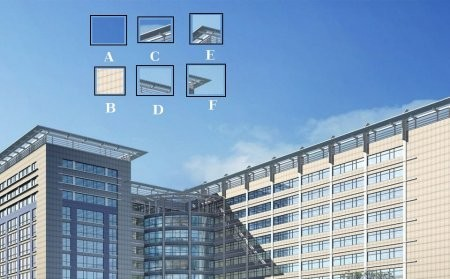
\includegraphics[width=0.7\textwidth]{features}
	\caption[Puntos de interés]{Ejemplo de caracterización de puntos en una imagen}
	\label{imagen:features}
\end{figure}

Atendiendo a la imagen \ref{imagen:features}, se puede observar que se caracterizan seis áreas de interés. Analizando estos segmentos, vemos que \textbf{\textit{A}} y \textbf{\textit{B}} corresponden con superficies planas, lo que hace que sea muy difícil identificar la ubicación exacta de estas superficies en la imagen original. Por otro lado, tenemos las regiones \textbf{\textit{C}} y \textbf{\textit{D}}, las cuales corresponden con bordes en la imagen, si bien, se puede limitar en gran medida el área de búsqueda hacia toda las regiones del mismo bordes, sigue siendo difícil encontrar la ubicación exacta. Por ultimo, analizando las regiones \textbf{\textit{E}} y \textbf{\textit{F}} tenemos que corresponden a esquinas de la imagen original, en este caso se puede identificar fácilmente la ubicación exacta de la región en la imagen.

A partir de esta idea, en la cual se consideran las esquinas como regiones fácilmente identificables en una imagen, en \textit{1988} nace el primer algoritmo de detección de puntos de interés llamado Detector de esquinas de Harris \cite{harris} (nombre original en inglés: Harris Corner Detector), y como su nombre lo indica está basado en la detección de esquinas.

Retomando el concepto planteado previamente, este detector busca la diferencia de intensidad en una ventada de exploración cuando es desplazada en diferentes direcciones. Es decir, se detectará una esquina, para aquellas regiones que presenten una alta variación de intensidad al desplazar la ventana estudiada en cualquier dirección. En la figura \ref{imagen:harris-window} se puede apreciar visualmente como funciona esta ventana de búsqueda.

\begin{figure}[H]
	\centering
	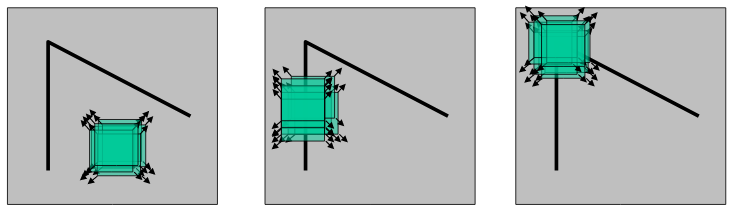
\includegraphics[width=0.9\textwidth]{harris-window}
	\caption[Deteccion de esquinas]{Desplazamiento de la ventana de búsqueda, para de detección de esquinas}
	\label{imagen:harris-window}
\end{figure}

Cuando se trabajan con detectores de características, se desea que estos sean invariantes ante la mayor cantidad de variables posibles, es decir, que sean capaces de detectar las mismas características en una imagen a pesar de cambios en la traslación, rotación, escala, variaciones de iluminación, variaciones del punto de vista, e incluso deformaciones debido a transformaciones geométricas. Si bien el detector presentado anteriormente es invariante ante la traslación y la rotación (ya que las esquinas se mantienen como esquinas si son rotadas o desplazadas), no funciona de la misma forma ante cambios de escala. Como se observa en la figura \ref{imagen:corner-scale}, una región considerada como esquina, se podría considerar plana si es ampliada.

\begin{figure}[H]
	\centering
	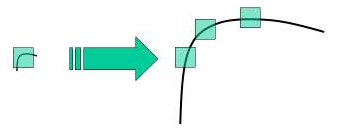
\includegraphics[width=0.85\textwidth]{corner-scale}
	\caption[Deteccion de esquinas]{Desplazamiento de la ventana de búsqueda, para de detección de esquinas}
	\label{imagen:corner-scale}
\end{figure}

Otra característica que se busca en estos algoritmos para lograr ubicar estas características ya detectada en una imagen distinta, es la que tengan la capacidad de realizar una descripción de estas regiones. Para esto, se desarrollaron los algoritmos descriptores, los cuales una vez tengan la ubicación de los puntos característicos se encargan de convertir la información de su alrededor en una serie de números, o un vector que permita diferenciar un punto clave de otro. Esta información también es necesaria que sea invariante ante las variable mencionadas previamente, para lograr una identificación eficiente del mismo punto en distintas imágenes.

Partiendo de estos problemas, en \textit{2004 D. Lowe} crea el detector y descriptor \textit{SIFT} \cite{sift} (del inglés: Scale Invariant Feature Transform), el cual presenta la innovación de poseer invarianza ante cambios en la escala. El proceso para la detección y descripción de puntos de interés de este algoritmo, consta de cuatro pasos principales:

En primer lugar, realiza una detección de máximos en el espacio de la escala aplicando la diferencia gaussiana \textit{DoG} (del inglés: Difference of Gaussians). Para esto, se aplica el filtro gaussiano con distintos tamaños de media (se tienen distintas escalas), luego restando estas imágenes para distintos pares de escalas se logra la diferencia de gaussianas. Posteriormente se buscan los máximos locales a lo largo del espacio (coordenadas X,Y) para cada correspondiente escala. Este proceso de detección se puede visualizar en la figura \ref{imagen:sift-escalas}.

\begin{figure}[H]
	\centering
	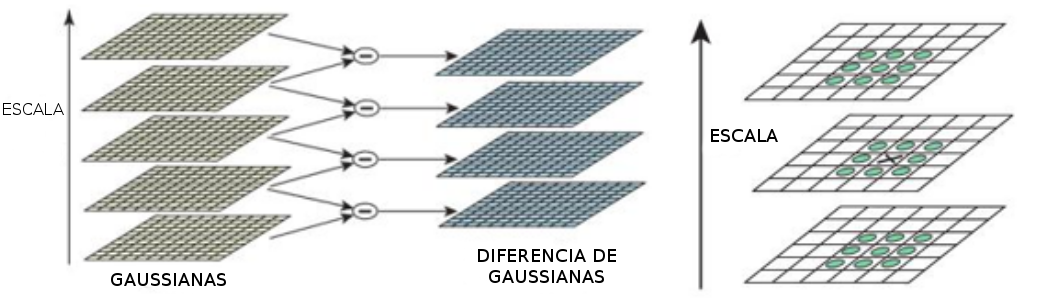
\includegraphics[width=0.85\textwidth]{sift-escalas}
	\caption[SIFT - Espacio de escalas]{Detección de máximos en el espacio de la escala}
	\label{imagen:sift-escalas}
\end{figure}

En segundo lugar para la localización de puntos de interés, se descartan los puntos encontrados en el paso anterior que no superen cierto valor de umbral, es decir, que no estén lo suficientemente contrastados con su entorno. Con esta etapa el algoritmo solo toma en cuenta los puntos claves mas fuertes por cada escala. Además, con el objetivo de eliminar los bordes suficientemente contrastados que no correspondan con esquinas, el algoritmo usa una matriz hessiana para calcular las curvaturas principales, y así quedarse solo con esquinas.

Para garantizar la invarianza con respecto a la rotación, se toman los píxeles vecinos al punto clave y se calcula la magnitud y dirección del gradiente en esa región. Con esto se hace un histograma de la magnitud del gradiente en cada dirección, donde el pico mayor del histograma indica la orientación. En el caso que exista un pico mayor al 80\% del pico principal, este se utiliza para crear otro punto de interés en la misma posición pero con la distinta rotación.

Finalmente para la descripción por cada punto clave se crea una matriz de 16x16 alrededor de este, dividida en 4 subregiones de 4x4 píxeles con un histograma de orientaciones para cada uno. Seguidamente, el descriptor del punto será el vector con los valores de los histogramas de las regiones 4x4 concatenados.

En el año 2006, un grupo de tres  personas Bay, H., Tuytelaars, T. and Van Gool, L. desarrollan \textit{SURF} \cite{surf}, el cual es un detector y descriptor de características basado en SIFT, pero con modificacioes que aumentan su velocidad de detección. Si bien, sacrifica un poco de rendimiento y precisión, lo hace mas provechoso para aplicaciones embebidas que demanden mayor velocidad de computo y menor uso de recursos, como por ejemplo \textit{SLAM} (del ingles: Simultaneous Localization and Mapping). El proceso para la extracción de características por parte de este algoritmo se compone de los siguientes pasos:

Como primer paso, en lugar de aproximar el laplaciano de Gauss \textit{LoG} (del inglés: Laplacian of Gaussians) con la diferencia de Gaussianas (DoG) como lo hace SIFT, este algoritmo aproxima LoG con cuadrados para promediar la imagen. La ventaja de aplicar filtros con cuadrados es que con la ayuda de imágenes integrales el cálculo computacional se reduce en gran medida.

\begin{figure}[H]
	\centering
	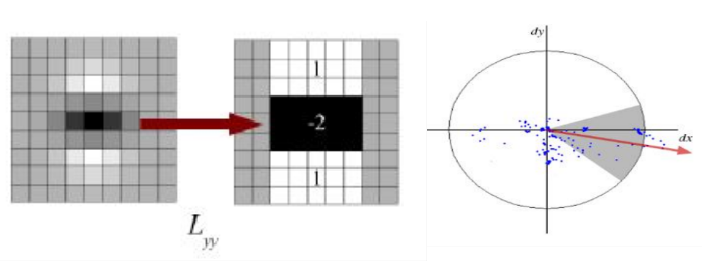
\includegraphics[width=0.8\textwidth]{surf}
	\caption[SURF - Espacio de escalas]{Detección de máximos en el espacio de la escala}
	\label{imagen:surf}
\end{figure}

En función de identificar la orientación, el algoritmo utiliza la respuesta wavelet Haar en horizontal y vertical en un vecindario de 6$s$ (donde $s$ es la escala evaluada) píxeles al rededor del punto de interés, Luego estas respuestas son representadas como puntos en el espacio, para luego calcular la orientación dominante con la suma de todos los resultados dentro de una ventana deslizante de apertura 60$^\circ$. En la figura \ref{imagen:surf} se puede visualizar la forma del filtro que aplica el detector, y el vector de orientación en función a la distribución de puntos estudiados.

El siguiente avance importante en los algoritmos de detección aparece en el año 2011 con \textit{ORB} \cite{orb} (del inglés: Oriented FAST and Rotated BRIEF), este utiliza una combinación del detector FAST (del inglés: Features from Accelerated Segment Test) y del descriptor BRIEF (del inglés: Binary Robust Independent Elementary Features), este nuevo algoritmo esta caracterizado por su alta velocidad de procesamiento manteniendo un buen rendimiento, gracias al uso de un descriptor binario. 

Como se mencionó utiliza el algoritmo FAST el cual consiste en encontrar esquinas evaluando los píxeles en un perímetro circular, de esta forma, un punto será detectado como esquina si la cantidad de píxeles de color opuesto al evaluado, supera cierto valor de umbral (ver izquierda en la figura \ref{imagen:orb}), posteriormente con el fin de aumentar la robustez, es aplicado el algoritmo de clasificación de esquinas de $Harris$. De igual forma se realiza con una estructura piramidal evaluando varias escalas (al igual que SIFT).

\begin{figure}[H]
	\centering
	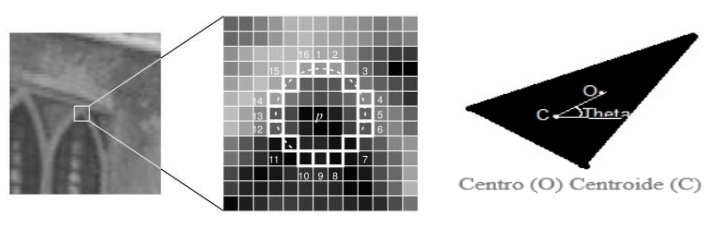
\includegraphics[width=0.9\textwidth]{orb}
	\caption[ORB - Espacio de escalas]{Detección de máximos en el espacio de la escala}
	\label{imagen:orb}
\end{figure}

Como el algoritmo FAST no toma en cuenta la orientación, en el ORB se modificó para que calculara la orientación de la siguiente forma: Se considera una región ubicada en el centro del punto estudiado, luego se calcula el centroide de la región en función a la intensidad de los puntos. De esta forma, la dirección del vector desde el punto central  hasta el centroide es asignado como vector de orientación. Observando a la derecha en \ref{imagen:orb} se aprecia un ejemplo del lugar del centroide \textit{(C)} y del centro \textit{(O)} par auna región en particular.


Para el descriptor utiliza BRIEF, a diferencia de los anteriores (SIFT y SURF) este es un descriptor binario y no vectorial. El descriptor BFIEF produce una palabra de $n$-bits usando el algoritmo \textit{Local Binay Tests} (LBT), el problema de esta representación es que no es muy robusta ante cambios en la rotación. Para resolver esto ORB utiliza la información de la orientación previamente calculada en el paso de detección para aplicar LBT en esa orientación.

Los algoritmos de detección que se mencionaron hasta este momento tienen una caracteristica en común, y es que cuando trabajan con el esquema piramidal lo hacen bajo el espacio de escala Gaussiano, el cual es una instancia particular de difusion lineal. De esta forma, al utilizar este filtro no se respetan los limites naturales de los objetos y se difumina del mismo nivel toda la region de la imagen cuando se avanza entre nieveles de escala.

Enfocándose en esta característica, en el año de \textit{2012} se desarrolla el detector y descriptor llamado KAZE \cite{kaze} por parte de \textit{Pablo Fernández Alcantarilla}. Este novedoso algoritmo opera completamente en un espacio de escala no lineal, para ello utilizan un esquema de división de operadores aditivos (\textit{AOS}, del inglés: Additive Operator Splitting), que les permite obtener espacios de escala no lineales de forma eficiente. De este modo se puede realizar un difuminado localmente adaptativo, posibilitando que se remueva el ruido en las imágenes, manteniendo información importante sobre los bordes de los objetos al avanzar en el espacio de escala. En la figura \ref{imagen:kaze} se puede observar como afecta en los bordes de los objetos el aplicar un filtro de difusión lineal, y uno que no lo es, bajo el esquema propuesto por este algoritmo.

\begin{figure}[H]
	\centering
	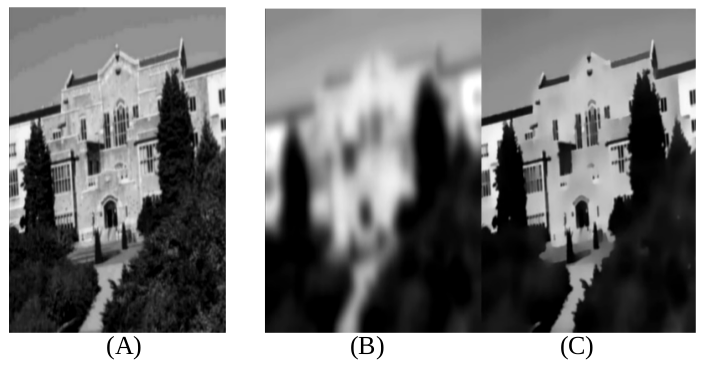
\includegraphics[width=0.85\textwidth]{kaze}
	\caption[KAZE - Espacio de escalas]{Deteccion de maximos en el espacio de la escala}
	\label{imagen:kaze}
\end{figure}

Bajo este mismo esquema de difusión no lineal, el mismo autor en el año \textit{2013} desarrolla la versión acelerada de este algoritmo que recibe el nombre de \textit{A-KAZE} \cite{akaze} (del ingles: Accelerated KAZE). Esta mejora se utiliza un esquema basado en difusión explícita rápida \textit{FED} (del ingles: Fast Explicit Difussion) en lugar de \textit{AOS}, el cual es un nuevo esquema piramidal que incrementa en gran medida la velocidad de computo para construir el espacio de escala no lineal.

Para el calculo de la orientación el primer algoritmo \textit{KAZE} utiliza un descriptor para la orientación similar al que emplea SURF. Este encuentra la orientación dominante en un área circular de radio 6$s$ ($s$ corresponde con la escala), y para cada muestra del círculo se calcula la derivada de primer orden en las direcciones $X$ e $Y$, y se ponderan con una gaussiana centrada en el punto de interés. Luego, las respuestas de estas derivadas son representadas como puntos en un espacio vectorial, donde la orientación dominante se haya sumando las respuestas dentro de un segmento de circulo deslizante con apertura de 60$^\circ$.

Por otro lado, la versión acelerada \textit{A-KAZE} emplea un descriptor basado en una versión modificada del algoritmo de diferencia local binaria \textit{LDB} \cite{ldb} (del ingles: Local Difference Binary), llamado M-LBD (del ingles: Modified Local Difference Binary), el cual aprovecha al máximo la información del espacio de escala no lineal. La modificación consiste en hacer un sub-muestreo de cada región que divide la zona del descriptor, en lugar de calcular el promedio de todos los píxeles de la región, es decir, se tienen muestras de cada subdivisión para distintas escalas.

\section{Proyección de imágenes}

 \begin{figure}[H]
 	\centering
 	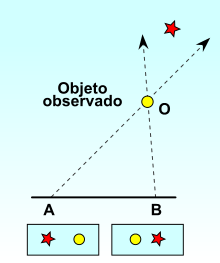
\includegraphics[width=0.85\textwidth]{paralaje1}
 	\caption[Paralaje - Efectos en el cambio de punto de vista]{Efectos en el cambio del punto de vista.}
 	\label{imagen:paralaje}
 \end{figure}
 
 Desde el punto de vista \textbf{A}, se observa la estrella a la izquierda del circulo. Mientras que desde le punto \textbf{B} la estrella es observada a la derecha del circulo.

\section{Fusión de imágenes}

mensaje de prueba 2

